\chapter{Renormalization in Information Theory}\label{sec:rsmi}
In the previous chapter, we used information theory to formalize the
notion of \textit{relevant} information. In this chapter, we will
adapt this to our physical context of long-distance as relevant
information. Ultimately, this allows us to devise a cost-function that
measures the physical information. From this, we can derive a learning
rule to train RBMs to perform \textit{optimal} transformations.

In the previous chapter, we saw that the Ising model's locality and
translational invariance conditions reduce the number of acceptable RG
procedures. Rather than devise an update rule for how an entire
configuration should transform under RG, we can start with
\fref{eq:prob-block-rg}.  Then, we only need to learn the
transformation for a single block, $P(h_j\rvert \bv^{(j)})$. We
already know that we can model conditional probabilities like these
with RBMs. This is the first insight of Koch-Janusz and Ringel, and in
this chapter, we will follow their information-theoretic
treatment~\cite{kjr}.

\section{An Information-Theoretic Formulation of RG}
First, we partition a full lattice configuration $\bx$ into four
areas: a visible block, $\bv$, that is surrounded by, in order, a
buffer, $\bb$, an environment, $\be$, and an outer area, $\bo$
\sref{fig:rsmi-overview}. In RG, we introduce a hidden area,
$\bh\eqcolon\{h_i\}$ which is a function of the degrees of freedom in
$\bv$. Our aim is to choose this coupling, $P(\bh\rvert\bv)$, so that
$\bh$ encodes the long-distance degrees of freedom about our system at
large, $\bx$\footnote{We have dropped the indices for convenience, and
  now we let block $\bh$ consist of multiple coarse-grained
  spins.}. By our assumption that $\bo$ is farther than the
correlation length, $\bv$ contains no information about $\bo$. We can
ignore $\bo$ in devising $P(\bh\rvert\bv)$. Furthermore, in coming up
with a function for $\bh$, we can reasonably ignore $\bb$. The
information contained in $\bv$ about $\bb$ is likely to be
short-range. By eliminating $\bb$, we throw out the shortest-range
fluctuations.
\begin{figure}[ht]
  \centering 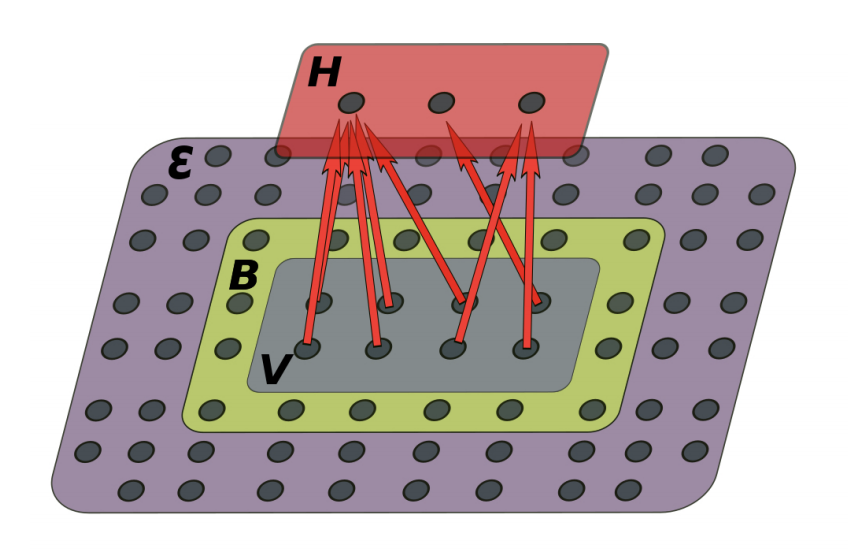
\includegraphics[width=0.5\textwidth]{figures/kjr.png}
  \caption{The RSMI algorithm partitions configurations into four
    regions, a visible block $\bv$, buffer zone $\bb$, environment
    $\be$ and outer zone, $\bo$. We introduce a coarse-grained block
    of spins $\bh$.\label{fig:rsmi-overview} }
\end{figure}%
That which remains is the physically relevant information; we see it
is the information shared between $\bv$ and $\be$. Our goal is to
extract this information and encode in $\bh$. We choose the
parameters, $\L$, of our RBM that models $P(\bh\rvert\bv)$ to maximize
the mutual information between $\bh$ and $\be$:%
\begin{equation}%
  I(\bh; \be)=\sum_{\bh,\be}P(\bh,\be)\log\left(\frac{P(\bh,\be)}{P(\bh)P(\be)}\right),\label{eq:rsmi}
\end{equation}%
where these probabilities are defined as marginalizations over
$P(\bx)$:%
\begin{align}%
  P(\bh, \be)&=\sum_{\bv}P(\bh\rvert \bv)P(\bv,\be)\\
  P(\bh)&=\sum_{\bv,\be}P(\bh\rvert \bv)P(\bv,\be)\\
  P(\bv,\be)&=\sum_{\bb,\bo}P(\bx)\\
  P(\be)&=\sum_{\bb,\bv,\bo}P(\bx).
\end{align}%

From previous chapters, we know that the probability measure $P(\bx)$
and its marginalizations are generally intractable. The key insight of
Koch-Janusz and Ringel is that we can use RBMs not only to model
$P(\bh\rvert \bv)$ but also to model these other
distributions. Koch-Janusz and Ringel ultimately use three RBMs: one
for $P(\bv,\be)$, another for $P(\bv)$, and finally the
$P(\bh\rvert\bv)$ RBM already mentioned. The other distributions are
calculated as MC-averages over the dataset. Hereby, Koch-Janusz and
Ringel derive a proxy to the mutual information \sref{sec:rsmi-calc}
which they can optimize with stochastic gradient descent.

To validate their ideas, they provide both experimental and
theoretical justification. For the 1D Ising model, these
marginalizations can be calculated exactly, and they show that
maximizing the RSMI rederives decimation, an RG procedure known to be
\textit{optimal} for the 1D Ising model in that the procedure does not
increase the range of the coarse-grained Hamiltonian.  In follow-up
research, Lenggenhager et al. (along with the aforementioned authors)
show that RSMI coarse-graining is more generally optimal, maintaining
short-distance in any number of dimensions. They further show this
holds even in some cases that the mutual information is not fully
saturated.  We direct the interested reader to~\cite{kjr}
and~\cite{lenggenhager} for these results.  In the remainder of this
capstone, we discuss our own implementation and generalization.

\paragraph{Measuring Critical Exponents}
Having trained an RBM according to the RSMI algorithm, we can use
finite-size scaling \sref{sec:finite-size-scaling} to estimate,
finally, critical exponents. An important detail will be to devise a
``thermometer'' that can measure the effective temperature at
successive RG-iterations. We discuss several options in
\fref{sec:thermometer}. These options, moreover, are intrinsic and do
not require explicit knowledge of the temperature. This means the RSMI
algorithm is fully unsupervised. If we encounter new systems where we
do not know the proper RG transformations (or even how to measure
``temperature''), then unsupervised approaches might save us
considerable headache. Rather than guess and check possible
transformations, we would first machine learn a renormalization
procedure on the system, then, observe and interpret, only later
attempting more calculation-heavy approaches. As Koch-Janusz and
Ringel put it, the RSMI algorithm could form the basis of the
``physical reasoning process'' itself~\cite{kjr]}. Instead of retroactively
explaining trends in our data, ML would proactively guide our
exploration.
